\documentclass[aspectratio=169,10pt,xcolor=table]{ctexbeamer}
\usetheme{Madrid}
\usecolortheme{seagull}

% --- 颜色定义 ---
\definecolor{coffee}{RGB}{68,48,36}
\definecolor{latte}{RGB}{226,214,200}
\definecolor{mocha}{RGB}{120,90,70}
\setbeamercolor{palette primary}{fg=latte,bg=coffee}
\setbeamercolor{palette secondary}{fg=latte,bg=mocha}
\setbeamercolor{palette tertiary}{fg=latte,bg=coffee}
\setbeamercolor{structure}{fg=coffee}
\setbeamercolor{titlelike}{fg=latte,bg=coffee}
\setbeamercolor{block title}{fg=latte,bg=mocha}
\setbeamercolor{block body}{fg=black,bg=latte!30}
\setbeamertemplate{title page}[default][colsep=-4bp,rounded=true]
\setbeamertemplate{navigation symbols}{}
\setbeamertemplate{caption}[numbered]
\setbeamertemplate{footline}[frame number]
\setbeamertemplate{itemize items}[circle]
\setbeamertemplate{enumerate items}[default]
% 参考文献样式
\bibliographystyle{unsrt}
\setbeamertemplate{bibliography item}[text]

% --- 宏包 ---
\usepackage{amsmath,amssymb,siunitx,booktabs,multirow,gensymb}
\usepackage{graphicx}
\usepackage{tikz}
\usetikzlibrary{arrows.meta,positioning,calc,shapes.geometric,shadows}
\usepackage{algorithm}
\usepackage{algpseudocode}
\floatname{algorithm}{算法}
\renewcommand{\algorithmicrequire}{\textbf{输入:}}
\renewcommand{\algorithmicensure}{\textbf{输出:}}

% --- 代码美化 ---
\usepackage[most]{tcolorbox}
\usepackage{listings}
\tcbuselibrary{listings}

\definecolor{pyblue}{RGB}{0,102,204}
\definecolor{pygreen}{RGB}{0,128,0}
\definecolor{pyred}{RGB}{204,0,0}
\definecolor{pybg}{RGB}{248,248,248}

\tcbset{
    codebox/.style={
        enhanced,
        colback=pybg,
        colframe=coffee!80!black,
        listing only,
        boxrule=0.5pt,
        arc=2pt,
        left=2pt, right=2pt, top=0pt, bottom=0pt,
        fonttitle=\bfseries\small,
        coltitle=white,
        sharp corners,
        drop shadow={shadow scale=1.05, shadow xshift=0.5pt, shadow yshift=-0.5pt}
    }
}

\newtcblisting{pythoncode}[1][]{
    codebox,
    colframe=pyblue!70!black,
    colbacktitle=pyblue,
    listing options={
        language=Python,
        basicstyle=\ttfamily\scriptsize,
        keywordstyle=\color{pyblue}\bfseries,
        stringstyle=\color{pyred},
        commentstyle=\color{pygreen}\itshape,
        numbers=none,
        breaklines=true,
        xleftmargin=2pt,
    },
    title={#1}
}

\title{\bfseries RV/少齿差减速器振动、精度与刚度理论建模}
\author{理论模型}
\date{\today}

\begin{document}

\begin{frame}
  \titlepage
\end{frame}

\begin{frame}{目录}
  \tableofcontents
\end{frame}

% ============================================================================ 
\section{研究背景与目标}
% ============================================================================ 

\begin{frame}{研究背景}
  \begin{columns}
    \begin{column}{0.6\textwidth}
      \begin{block}{核心部件：RV 与少齿差减速器}
      \begin{itemize}
        \item \textbf{应用领域}：工业机器人、数控机床、航空航天。
        \item \textbf{性能指标}：定位精度、重复精度、动态响应。
      \end{itemize}
      \end{block}
      
      \vspace{1em}
      \textbf{结构特点：}
      \begin{itemize}
        \item \textbf{少齿差传动}：内啮合渐开线齿轮副，齿数差 $1\sim4$ 齿。结构紧凑，通过偏心机构实现大传动比~\cite{litvin}。
        \item \textbf{RV 减速器}：两级传动（行星+摆线针轮）。摆线轮与针齿壳形成多点同时接触，具有高刚度、低回差~\cite{rvdynamic}。
      \end{itemize}
    \end{column}
    \begin{column}{0.4\textwidth}
      \centering
      \begin{tikzpicture}[scale=0.6]
         \draw[thick,fill=latte!30] (0,0) circle (2.5);
         \draw[thick,fill=white] (0.5,0) circle (1.5);
         \node at (0,2.8) {\small 内齿圈};
         \node at (0.5,0) {\small 外齿轮};
         \node at (0,-3) {\small 少齿差结构示意};
         \draw[->,dashed] (0,0) -- (0.5,0) node[midway,above] {\scriptsize $e$};
      \end{tikzpicture}
    \end{column}
  \end{columns}
\end{frame}

\begin{frame}{研究目标与技术路线}
  \begin{columns}[T]
    \begin{column}{0.48\textwidth}
      \textbf{研究目标：}
      \begin{enumerate}
        \item \textbf{振动特性}：固有频率、模态振型与强迫振动响应。
        \item \textbf{传动精度}：量化传递误差、回程误差与动态定位精度。
        \item \textbf{啮合刚度}：获取时变啮合刚度曲线，分析刚度波动。
        \item \textbf{参数优化}：支持齿廓修形、间隙补偿设计。
      \end{enumerate}
    \end{column}
    \begin{column}{0.48\textwidth}
      \textbf{关键技术：}
      \begin{enumerate}
        \item \textbf{解析几何表达}：无网格渐开线/摆线参数方程。
        \item \textbf{时变刚度建模}：Weber-Banaschek + Hertz 理论~\cite{johnson}。
        \item \textbf{专用接触模型}：FewTeeth (内啮合), CurveCircles (摆线)。
        \item \textbf{高效接触搜索}：角度筛选、AABB、Warm-start。
      \end{enumerate}
    \end{column}
  \end{columns}
\end{frame}

% ============================================================================ 
\section{少齿差齿轮建模}
% ============================================================================ 

\begin{frame}{少齿差齿轮几何参数}
  \begin{columns}[T]
    \begin{column}{0.5\textwidth}
      \textbf{基本参数 (FewTeethGearPair):}
      \begin{table}
      \small
      \rowcolors{2}{latte!20}{white}
      \begin{tabular}{ll}
      \toprule
      符号 & 说明 \\
      \midrule
      $z_1, z_2$ & 齿数 ($z_2 = z_1 + \Delta z$) \\
      $m$ & 模数 \\
      $\alpha$ & 压力角 (标准 $20^\circ$) \\
      $x_1, x_2$ & 变位系数 \\
      $h_a^*, c^*$ & 齿顶高/顶隙系数 \\
      \bottomrule
      \end{tabular}
      \end{table}
      
      \textbf{数据节点 (7变量状态向量):}
      \begin{equation*}
        \mathbf{D}_{node} = [g, \dot{g}, f_n, idx_{out}, u_{out}, idx_{in}, u_{in}]^T
      \end{equation*}
    \end{column}
    \begin{column}{0.5\textwidth}
      \textbf{导出几何量：}
      \small
      \begin{align}
      r &= \frac{m z}{2}, \quad r_b = r \cos\alpha \\
      r_a &= r + m(h_a^* + x) \\
      r_f &= r - m(h_a^* + c^* - x) \\
      a_0 &= \frac{m(z_2 - z_1)}{2} \frac{\cos\alpha}{\cos\alpha_0}
      \end{align}
      其中 $\alpha_0$ 为啮合角。
    \end{column}
  \end{columns}
\end{frame}

\begin{frame}{渐开线齿廓解析表达}
  \textbf{无网格参数化方法：}
  引入参数 $u \in [0, 1]$ 描述从齿根圆 $r_{\min}$ 到齿顶圆 $r_{\max}$ 的位置。
  
  \begin{columns}
    \begin{column}{0.6\textwidth}
      \small
      \begin{align}
      r(u) &= r_{\min} + u (r_{\max} - r_{\min}) \\
      \alpha_c &= \arccos(r_b / r) \\
      \theta_c &= \tan\alpha_c - \alpha_c \quad (\text{inv function}) \\
      \phi_c &= \begin{cases}
        \theta_{base} + \phi_{pitch} - \theta_c & (\text{外齿}) \\
        -\theta_{base} + \phi_{pitch} + \theta_c & (\text{内齿})
      \end{cases}
      \end{align}
      \vspace{-1em}
      \begin{equation}
      x = r \sin\phi_c, \quad y = r \cos\phi_c
      \end{equation}
    \end{column}
    \begin{column}{0.4\textwidth}
      \centering
      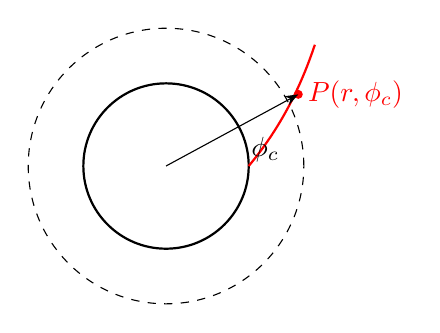
\begin{tikzpicture}[scale=0.7,>=Stealth]
        \draw[thick] (0,0) circle (1.5); % Base
        \draw[dashed] (0,0) circle (2.5); % Pitch
        \draw[red,thick] (1.5,0) .. controls (2.0,0.6) and (2.4,1.3) .. (2.7,2.2);
        \filldraw[red] (2.4,1.3) circle (2pt) node[right] {$P(r,\phi_c)$};
        \draw[->] (0,0) -- (2.4,1.3);
        \node at (1.8,0.3) {$\phi_c$};
      \end{tikzpicture}
    \end{column}
  \end{columns}
\end{frame}

\begin{frame}{FewTeeth 多级接触搜索算法}
  为提高计算效率，采用四级筛选策略，将复杂度从 $O(N^2)$ 降至 $O(N)$：
  
  \begin{enumerate}
      \item \textbf{角度预筛选 (Angle Filter)}：
      \begin{itemize}
          \item 右齿面：仅检测滞后区 $\theta \in [-45^\circ, 0^\circ]$。
          \item 左齿面：仅检测超前区 $\theta \in [0^\circ, 45^\circ]$。
      \end{itemize}
      
      \item \textbf{活跃集热启动 (Warm-start)}：
      \begin{itemize}
          \item 利用时间连续性，优先检测上一时间步活跃的齿对 $(idx_{out}, idx_{in})$。
      \end{itemize}
      
      \item \textbf{解析求解 (Analytic Solver)}：
      \begin{itemize}
          \item 在外齿轮齿面采样（如36点），计算到内齿轮的最小距离平方。
      \end{itemize}
      
      \item \textbf{探针回退 (Tip Probe)}：
      \begin{itemize}
          \item 当解析求解失效（如齿尖区），从齿尖发射射线与内齿廓求交。
      \end{itemize}
  \end{enumerate}
\end{frame}

% ============================================================================ 
\section{摆线针轮建模}
% ============================================================================ 

\begin{frame}{摆线齿廓方程}
  基于短幅外摆线理论生成齿廓~\cite{cycloidmodel}，包含修形参数 $\delta$：
  
  \scriptsize
  \begin{align}
    x(\phi) &= -\left[(R_p - \delta_{R_p}) - \frac{r_p + \delta_r}{\sqrt{S'}}\right]\sin\left[(1-i_H)\phi - \delta\right] 
    - \frac{a}{R_p - \delta_{R_p}}\left[(R_p - \delta_{R_p}) - \frac{z_p(r_p + \delta_r)}{\sqrt{S'}}\right]\sin(i_H\phi + \delta) \\
    y(\phi) &= \left[(R_p - \delta_{R_p}) - \frac{r_p + \delta_r}{\sqrt{S'}}\right]\cos\left[(1-i_H)\phi - \delta\right] 
    - \frac{a}{R_p - \delta_{R_p}}\left[(R_p - \delta_{R_p}) - \frac{z_p(r_p + \delta_r)}{\sqrt{S'}}\right]\cos(i_H\phi + \delta)
  \end{align}
  \normalsize
  其中 $z_p$ 为针齿数，$a$ 为偏心距，$R_p$ 为分布圆半径，$r_p$ 为针齿半径，$S'$ 为辅助系数。
\end{frame}

\begin{frame}{Curve-Circles 高级接触算法}
  针对摆线轮与针齿列的一对多接触，引入增强算法：
  
  \begin{columns}[T]
    \begin{column}{0.5\textwidth}
      \textbf{1. 多项式几何增强：}
      为保证 $C^1/C^2$ 连续，对线段引入三次多项式修正：
      \small
      \begin{equation}
        y(x) = a_0 \phi_0(x) + a_1 \phi_1(x)
      \end{equation}
      其中 $\phi_i(x)$ 为形函数，利用端点斜率平滑过渡。
      
      \vspace{0.5em}
      \textbf{2. 面积积分接触模型：}
      为消除线段转折处的力突变，采用重叠区域积分：
      \small
      \begin{equation}
      f_n^{area} = \frac{f_n}{g} \int_{s_0}^{s_1} \left[ \sqrt{r^2 - d^2(s)} - d_0 \right] ds
      \end{equation}
    \end{column}
    \begin{column}{0.5\textwidth}
      \textbf{3. 等弧长重采样：}
      \begin{itemize}
          \item 积分弧长 $s(\phi)$，反解 $\phi_i$ 使得 $\Delta s = const$。
      \end{itemize}
      
      \vspace{0.5em}
      \textbf{4. 块跳过 (Block Skip)：}
      \begin{itemize}
          \item 若当前块（如8个线段）两端均远离圆心，直接跳过检测。
      \end{itemize}
      
      \centering
      \begin{tikzpicture}[scale=0.6]
        \draw[thick,blue] plot [smooth] coordinates {(0,0) (1,0.5) (2,0) (3,0.8)};
        \draw[fill=red!20] (1.5, 0.2) circle (0.4);
        \node at (1.5,-0.5) {\scriptsize 积分区域};
      \end{tikzpicture}
    \end{column}
  \end{columns}
\end{frame}

% ============================================================================ 
\section{啮合刚度与接触力学}
% ============================================================================ 

\begin{frame}{时变啮合刚度模型}
  啮合刚度 $k_{mesh}$ 是影响传动精度与振动的关键，采用串联刚度模型计算：
  \begin{equation}
    \frac{1}{k_{mesh}} = \frac{1}{k_{struct,1}} + \frac{1}{k_{struct,2}} + \frac{1}{k_{contact}}
  \end{equation}
  
  \vspace{0.5em}
  \begin{description}
      \item[$k_{struct}$ (结构刚度)] 包含齿体弯曲变形 $\delta_B$ 与齿根变形 $\delta_M$ (Ishikawa 公式)。
      \item[$k_{contact}$ (接触刚度)] 基于 Hertz 接触理论，随接触点曲率半径变化。
  \end{description}

  \centering
  \tikz[baseline=-0.5ex]{
    \node[draw,fill=latte!20,rounded corners] {弯曲 $\delta_B$}; 
  } + 
  \tikz[baseline=-0.5ex]{
    \node[draw,fill=latte!20,rounded corners] {剪切 $\delta_S$}; 
  } + 
  \tikz[baseline=-0.5ex]{
    \node[draw,fill=latte!20,rounded corners] {齿根 $\delta_M$}; 
  } + 
  \tikz[baseline=-0.5ex]{
    \node[draw,fill=mocha!20,rounded corners] {Hertz $\delta_C$}; 
  }
\end{frame}

\begin{frame}{结构刚度与接触刚度公式}
  \begin{columns}[T]
    \begin{column}{0.5\textwidth}
      \textbf{齿体弯曲 (Beam Theory):}
      \scriptsize
      \begin{equation}
      \delta_B = \frac{F}{E} \int \left[ \frac{M(x)^2}{I(x)} + \frac{F_N^2}{A(x)} + k \frac{F_S^2}{A(x)} \right] dx
      \end{equation}
      \normalsize
      \textbf{齿根变形 (Ishikawa):}
      \scriptsize
      \begin{equation}
      \delta_M \propto \frac{F}{E} \left[ \left(\frac{L_f}{H_f}\right)^2 + \frac{L_f}{H_f} + 1 \right]
      \end{equation}
    \end{column}
    \begin{column}{0.5\textwidth}
      \textbf{Hertz 接触刚度:}
      对于内-外齿啮合（凹-凸接触），等效曲率半径 $\rho_{eq}$：
      \begin{equation}
      \rho_{eq} = \frac{\rho_1 \rho_2}{|\rho_2 - \rho_1|}
      \end{equation}
      接触趋近量 $\delta_C$：
      \begin{equation}
      \delta_C = \frac{2F}{\pi B} \frac{1-\nu^2}{E} \left[ \ln\left(\frac{2\rho_{eq}}{b}\right) + 0.4 \right]
      \end{equation}
    \end{column}
  \end{columns}
\end{frame}

\begin{frame}{罚式接触力学模型与数值处理}
  采用基于穿透深度的非线性罚函数法，结合正则化技术保证稳定性：
  
  \begin{block}{法向接触力}
  \begin{equation}
   f_n = k_{mesh}(\theta) \cdot \max(0, -g)^{10/9} + d_c \cdot \max(0, -\dot{g})
  \end{equation}
  \end{block}
  
  \textbf{数值稳健性处理：}
  \begin{itemize}
      \item \textbf{不连续性处理 (PostNewtonStep)}：在牛顿迭代收敛后检测接触状态切换（分离$\leftrightarrow$接触），触发雅可比矩阵更新。
      \item \textbf{Stribeck 摩擦正则化}：
      \begin{equation}
        f_t = -\mu |f_n| \cdot \text{sgn}(v_t) \cdot \min(1, |v_t|/v_{reg})
      \end{equation}
  \end{itemize}
\end{frame}

% ============================================================================ 
\section{接触搜索与算法}
% ============================================================================ 

\begin{frame}{FewTeeth 接触求解流程}
\centering
\resizebox{0.9\textwidth}{!}{
\begin{tikzpicture}[node distance=1.2cm,>=Stealth,
  block/.style={rectangle,rounded corners,draw,align=center,fill=latte!80,minimum width=3.5cm,minimum height=0.8cm},
  decision/.style={diamond,aspect=2,draw,fill=mocha!40,align=center,inner sep=2pt},
  arrow/.style={->,thick,draw=coffee}]
  
  \node[block] (start) {读取位姿 $(\mathbf{q}, \dot{\mathbf{q}})$};
  \node[block,right=1cm of start] (filter) {角度预筛选/AABB};
  \node[block,right=1cm of filter] (eval) {解析齿廓求值 $(r,\phi)$};
  \node[decision,below=1cm of eval] (gap) {$g < 0$?};
  
  \node[block,below left=1cm and 0.5cm of gap] (stiff) {啮合刚度计算 $k_{mesh}$};
  \node[block,below=0.8cm of stiff] (force) {计算接触力 $f_n, f_t$};
  \node[block,below right=1cm and 0.5cm of gap] (probe) {探针回退检测};
  
  \node[block,below=3.5cm of gap] (assemble) {力装配 $\mathbf{f}_{contact}$};
  
  \draw[arrow] (start) -- (filter);
  \draw[arrow] (filter) -- (eval);
  \draw[arrow] (eval) -- (gap);
  \draw[arrow] (gap.west) -| node[above,pos=0.1]{Yes} (stiff.north);
  \draw[arrow] (gap.east) -| node[above,pos=0.1]{No} (probe.north);
  \draw[arrow] (stiff) -- (force);
  \draw[arrow] (force) |- (assemble);
  \draw[arrow] (probe) |- (assemble);
\end{tikzpicture}
}
\end{frame}

\begin{frame}{三类自定义接触模型对比}
  \begin{table}
  \centering
  \small
  \rowcolors{2}{latte!20}{white}
  \begin{tabular}{lccc}
  \toprule
  特性 & FewTeeth & CurveCircles & CircleCircle \\
  \midrule
  \textbf{几何表示} & 解析渐开线 & 分段线段+多项式 & 圆心+半径 \\
  \textbf{接触类型} & 凸-凹（内啮合） & 凸-凸/凹 & 凸-凸/凸-凹 \\
  \textbf{数据节点} & 7变量 ($g, f_n, idx...$) & 3变量 ($idx, g, v_t$) & 6变量 \\
  \textbf{刚度特性} & \textbf{时变+Hertz} & 常值/面积积分 & 常值 \\
  \textbf{搜索策略} & 4级筛选 (含探针) & AABB+块跳过 & 无需搜索 \\
  \textbf{摩擦模型} & 库仑 & Stribeck & 库仑 \\
  \bottomrule
  \end{tabular}
  \end{table}
\end{frame}

% ============================================================================ 
\section{后处理与结果分析}
% ============================================================================ 

\begin{frame}{结果分析与精度评估}
  \begin{columns}
    \begin{column}{0.5\textwidth}
      \textbf{1. 传递误差 (Transmission Error):}
      \begin{equation}
      TE(\theta) = \theta_{out} - \frac{\theta_{in}}{i}
      \end{equation}
      反映减速器的运动精度与波动。

      \vspace{0.5em}
      \textbf{2. 啮合刚度波动:}
      \begin{itemize}
          \item 监测 $k_{mesh}(t)$ 的时变特性。
          \item 分析刚度激励引起的振动响应。
      \end{itemize}
    \end{column}
    \begin{column}{0.5\textwidth}
      \textbf{3. 接触力分布:}
      \begin{itemize}
          \item 摆线轮各针齿的受力分布。
          \item 滚针轴承的载荷情况。
      \end{itemize}
      
      \vspace{0.5em}
      \textbf{4. 振动响应:}
      \begin{itemize}
          \item 输入/输出轴的角加速度频谱。
          \item 固有频率与模态分析。
      \end{itemize}
    \end{column}
  \end{columns}
\end{frame}

% ============================================================================ 
\section{参考文献}
% ============================================================================ 

\begin{frame}[allowframebreaks]{参考文献}
  \nocite{*}
  \bibliography{references}
\end{frame}

\end{document}